\chapter{Теорема Гаусса}

\section{Теорема Гаусса}
    
    Пусть в пространстве находится группа зарядов \( q_{n} \). Обхватим их 
    поверхностью \( S \). Так как группа зарядов создаёт поле \( \vec{E} \), то 
    через поверхность \( S \) поток поля может быть найден как
    \[
        \Phi = \oiint\limits_S \vec{E}\cdot\dd\vec{S}.
    \]
    Рассмотрим теорему, связывающую поток поля \( \vec{E} \) через замкнутую 
    поверхность \( S \) с зарядом, находящимся внутри поверхности.
    
    \begin{figure}[b]
        \center
        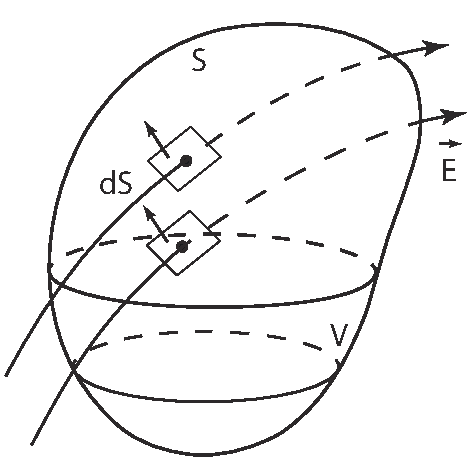
\includegraphics[width=0.30\textwidth]{lec02/flux_E.pdf}
        \hfill
        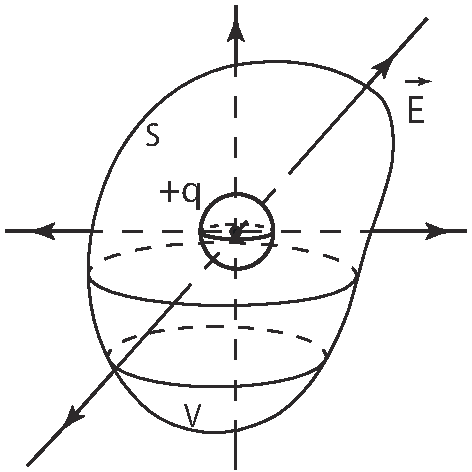
\includegraphics[width=0.30\textwidth]{lec02/Gauss_theorem.pdf} 
        \hfill
        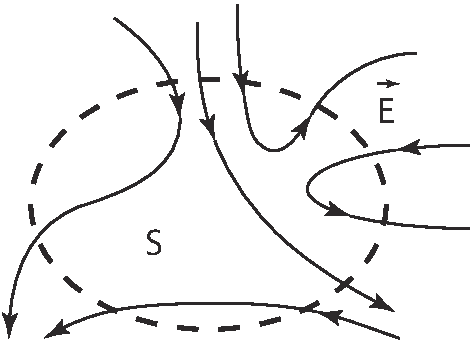
\includegraphics[width=0.30\textwidth]{lec02/Earnshaw_theorem.pdf}
        \parbox[t]{.3\textwidth}{
            \caption{Поток поля Е через поверхность S}
        }
        \hfill
        \parbox[t]{.3\textwidth}{
            \caption{К доказательству теоремы Гаусса}
        }
        \hfill
        \parbox[t]{.3\textwidth}{
            \caption{К доказательству теоремы Ирншоу}
        }
    \end{figure}
    

    \begin{theorem}[Гаусс]
        Поток поля \( \vec{E} \) через произвольную замкнутую поверхность
        \( S \) равен алгебраической сумме зарядов внутри \( S \), отнесённый к 
        \( \Ezero \), и не зависит ни от конфигурации зарядов, ни от формы
        \( S \).
        \begin{equation}
            \label{eq:thegauss}
            \Phi = \oiint\limits_S \vec{E}\cdot\dd\vec{S} = 
            \frac{\sum{q}}{\Ezero} = \frac{q_{S}}{\Ezero}
        \end{equation}
    \end{theorem}


    \begin{proof}
        Докажем сначала для одного заряда, затем применим принцип суперпозиции. 
        Так как заряд \( q \) является точечным изолированным источником поля 
        \( \vec{E} \), то, в силу следствия 2 теоремы Остроградского поток 
        через произвольную поверхность будет равен потоку через сферу радиуса 
        \( R \) в центре которой расположен заряд \( q \):
        \[
            \oiint\limits_S \vec{E}\cdot\dd\vec{S} = 
            \oiint\limits_{4\pi R^{2}} \vec{E}\cdot\dd\vec{S} = 
            \oiint\limits_{4\pi R^{2}}\frac{\vec{r}\cdot\dd\vec{S}}{r^3}
            \cdot\frac{q}{4\pi\Ezero}.
        \]

        А так как на сфере \( \vec{r} \uparrow\uparrow \dd\vec{S} \) и
        \( r = \const = R\), то
        \[
            \oiint\limits_{4\pi R^{2}}
            \frac{\vec{r}\cdot\dd\vec{S}}{r^3}\cdot\frac{q}{4\pi\Ezero} = 
            \frac{q}{4\pi\Ezero}\oiint\limits_{4\pi R^2} \frac{R\dd S}{R^3} = 
            \frac{q}{4\pi\Ezero R^2}\oiint\limits_{4\pi R^2}\dd S = 
            \frac{q}{\Ezero}.
        \]

        Если \( q \) лежит вне поверхности \( S \), то внутри \( S \)
        \( \div\vec{E} \equiv 0 \) и
        \[
            \Phi_{S} = \oiint\limits_S \vec{E}\cdot\dd\vec{S} = 
            \iiint\limits_V \div\vec{E}\dd V = 0.
        \]

        Итак, если внутри \( S \) содержится много зарядов, то в силу принципа 
        суперпозиции:

        \[
            \vec{E}=\sum\limits_k \vec{E}_{k},
        \]
        \[
            \Phi_{S} = \oiint\limits_S \vec{E}\cdot\dd\vec{S} =
            \sum\limits_k\oiint \vec{E}_{k}\cdot\dd \vec{S} =
            \sum\limits_k \frac{\pm q_{k}}{\Ezero} = \frac{q_{S}}{\Ezero}.
        \]

    \end{proof}

    Если заряд распределён в пространстве непрерывно, то
    \[
        q_{S} = \iiint\limits_V \rho(x,y,z)\dd V ,
    \]
    где \( \rho \) -- объёмная плотность заряда. Тогда теорема Гаусса даёт
    \[
        \oiint\limits_S \vec{E}\cdot\dd\vec{S} =             
        \frac{1}{\Ezero}\iiint\limits_V\rho\dd V,
    \]
    но, по теореме Остроградского,
    \[
        \oiint\limits_S \vec{E}\cdot\dd\vec{S} =
        \iiint\limits_V \div\vec{E}\dd V,
    \]
    таким образом,
    \[ 
        \iiint\limits_V \div\vec{E}\dd V =
        \frac{1}{\Ezero}\iiint\limits_V \rho\dd V,
    \]
    а так как область \( V \) произвольна, то подынтегральные значения равны:
    \begin{equation}
        \label{eq:thegaussdiff}
        \div\vec{E} = \frac{\rho}{\Ezero}.
    \end{equation}

    Формула (\ref{eq:thegaussdiff}) -- это дифференциальный вид
    (\ref{eq:thegauss}), она связывает поле \( \vec{E} \) и заряд в данной 
    точке.

\section{Теорема Ирншоу}

    \begin{theorem}[Ирншоу]
        Равновесие зарядов в электростатическом поле не может быть устойчивым.
    \end{theorem}

    \begin{proof}
        Пусть в поле \( \vec{E} \), созданном какими-либо внешними зарядами, 
        есть область устойчивости \( S \). Отсюда следует, что все линии 
        стабилизирующего поля \( \vec{E} \) входят в \( S \), но, так как в 
        области \( S \) зарядов нет, то, по теореме Гаусса,
        \[
            \oiint\limits_S \vec{E}\cdot\dd\vec{S} = 0,
        \]
        то есть сколько линий входит, столько и выходит. Таким образом 
        существуют траектории, выходящие за пределы области \( S \), движение 
        вдоль которых энергетически выгодно для заряда, находящегося в 
        состоянии равновесия в области, то есть его положение равновесия не 
        является устойчивым.
    \end{proof}

\section{Применение теоремы Гаусса}
    \begin{figure}[b]
        \center
        \subfigure[Поле плоскости]{
        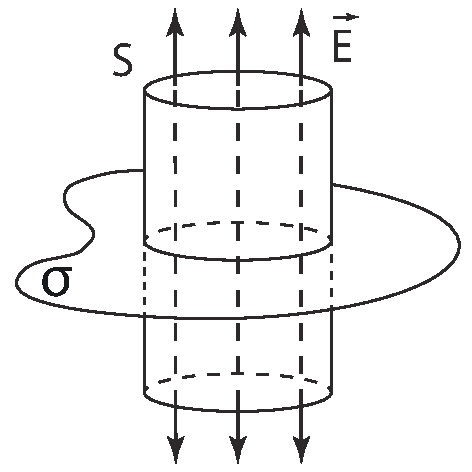
\includegraphics[width=0.30\textwidth]{lec02/plane_field.pdf} 
        \label{E_def}
        }
        \subfigure[Поле нити]{
        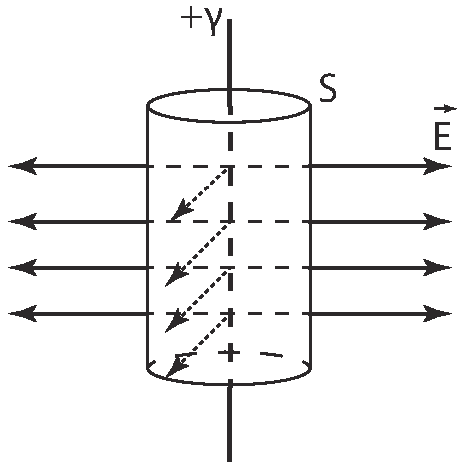
\includegraphics[width=0.30\textwidth]{lec02/thread_field.pdf}
        }
        \subfigure[Поле сферы]{
        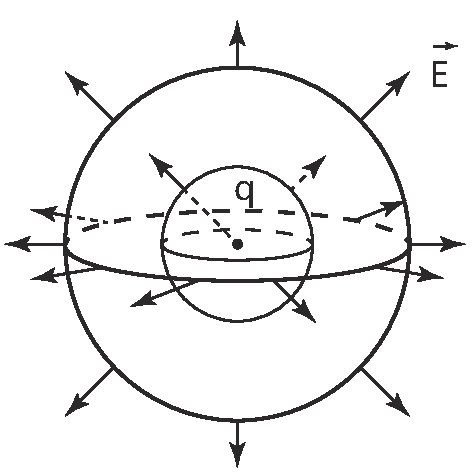
\includegraphics[width=0.30\textwidth]{lec02/sphere_field.pdf}
        }    
        \caption{Электрическое поле}
    \end{figure}
    
    \begin{figure}[b]
        \center
        \subfigure[Поле плоскости]{
            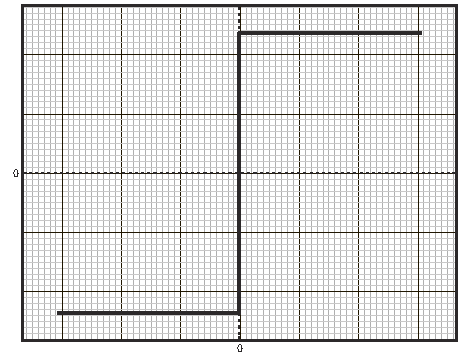
\includegraphics[width=0.3\textwidth]{lec02/plane_field_plot.pdf}
            \label{plane_field_plot}
        }
        \subfigure[Поле нити]{
            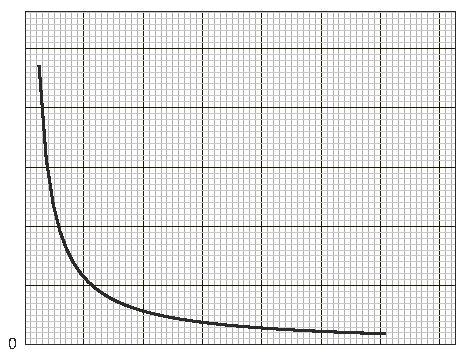
\includegraphics[width=0.30\textwidth]{lec02/thread_field_plot.pdf}
            \label{thread_field_plot}
        }
        \subfigure[Поле сферы]{
            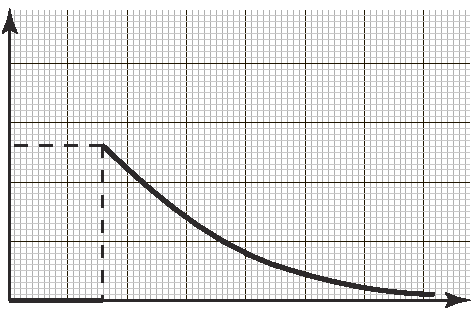
\includegraphics[width=0.30\textwidth]{lec02/sphere_field_plot.pdf}
            \label{sphere_field_plot}
        }
        \caption{Зависимости напряжённости поля от расстояния до системы}
    \end{figure}
    
    Теорема Гаусса, вообще говоря, не позволяет вычислить поле \( \vec{E} \) 
    заданной произвольной конфигурации зарядов, так как из знания интеграла 
    \( \Phi_S \) не следует знание \( \vec{E}(x,y,z) \). Однако, для некоторых 
    симметричных зарядовых конфигураций \( \Phi_S \sim ES \) и тогда теорема 
    Гаусса помогает считать значительно быстрее. 

    \begin{example}
        Вычислить поле \(\vec{E}\) бесконечной плоскости, на которой заряд 
        распределён равномерно с поверхностной плотностью
        \( \sigma\ (\text{Кл}/\text{м}^2) \).
    \end{example}


    \begin{solution}
        В силу симметрии объекта, поле \( \vec{E} \) плоскости может быть 
        только перпендикулярно плоскости. Поэтому найдём такое поле
        \( \vec{E} \).

        Обернём плоскость замкнутой поверхностью \( S \) в виде цилиндра, 
        перпендикулярного плоскости.
        \[
            S = S_{\textit{бок}} + 2S_{\textit{тор}}.
        \]

        Тогда, по теореме Гаусса,
        \[
            \oiint\limits_S \vec{E}\cdot\dd\vec{S} = \frac{q_{S}}{\Ezero},
        \]
        где \( q_{S} = \sigma\cdot S_{\textit{тор}} \) (заряд, вырезанный
        \( S \)).

        \[
            \Phi = \iint\limits_{S_{\textit{бок}}} \vec{E}\cdot\dd\vec{S} +
            2\iint\limits_{S_{\textit{тор}}} \vec{E}\cdot\dd\vec{S} =         
            2ES_{\textit{тор}}
        \]

        Таким образом,
        \[ 
            2ES_{\textit{тор}} = \frac{\sigma S_{\textit{тор}}}{\Ezero}
            \Rightarrow E = \frac{\sigma}{2\Ezero}
        \].

    \end{solution}

    \begin{example}
        Вычислить поле \( \vec{E} \) прямой бесконечной нити, равномерно 
        заряженной с погонной (линейной) плотностью
        \( \gamma\ (\text{Кл}/\text{м}) \).
    \end{example}

    \begin{solution}
        Охватим участок нити длины \( h \) соосным цилиндром радиуса \( r \). 
        Его площадь
        \[
            S = S_{\textit{бок}} + 2S_{\textit{тор}}.
        \]
        
        Так как поток поля через торцы равен 0 и
        \( \vec{E} \uparrow\uparrow \dd\vec{S} \), \( \vec{E} = \const \) на
        \( S_{\textit{бок}} \), то 
        \[
            \iint\limits_{S_{\textit{бок}}} \vec{E}\cdot\dd\vec{S} = 
            E\iint\limits_{S_{\textit{бок}}} \dd S = E\cdot 2\pi rh
        \]

        А так как цилиндр вырезает заряд \( q_{S} = \gamma h \), то, по теореме 
        Гаусса:
        \[
            E\cdot 2\pi rh = \frac{\gamma h}{\Ezero} \Rightarrow E = 
            \frac{\gamma}{2\pi\Ezero r}.
        \]
        В декартовых координатах:
        \[
            \vec{E}=\frac{\gamma}{2\pi\Ezero(x^2+y^2)}\cdot \{x, y, 0\}.
        \] 
    \end{solution}
    \begin{example}
        Вычислить поле \( \vec{E} \) сферы радиуса \( R \),
        несущей заряд \( q \).
    \end{example}
    \begin{solution}
        Сфера разделяет пространство на 2 части: внутреннюю и внешнюю по 
        отношению к сфере.
        \begin{enumerate}
        \item \( | \vec{r} | < R \) (внутри сферы).
            
            \( E_{in} \equiv 0 \), так как внутри любой сферической поверхности
            \( 4\pi r^2 \) (\( r < R \)) заряд \( q = 0 \).
            \[ \oiint\limits_{4\pi R^2} \vec{E}\cdot\dd\vec{S} = 0 \]

        \item \( | \vec{r} | > R \) (вне сферы).
      
            \[
                \oiint\limits_{4\pi R^2} \vec{E}\cdot\dd\vec{S} = 
                \frac{q_{S}}{\Ezero} = \frac{q}{\Ezero}.
            \]
            С другой стороны,
            \[
                \oiint\limits_{4\pi R^2} \vec{E}\cdot\dd\vec{S} =
                E_{ex}\cdot S_\textit{сф} =
                4\pi R^2 E_{ex} \Rightarrow \text{ при \( r > R\): }
                E = \frac{q}{4\pi\Ezero r^2}
            \]
        \end{enumerate} 

        Таким образом,
        \[ E = \frac{q}{4\pi\Ezero r^2} \].

        График этой зависимости изображён на рисунке~\ref{sphere_field_plot}.
        
    \end{solution}
